% !TEX root = main.tex

\section{Models}

\subsection{Logic Tensor Network (LTN)}

multilayer perceptron (MLP). The key differencen is that the first layer is not linear layer but bilinear layer.

\begin{figure}
    \centering
    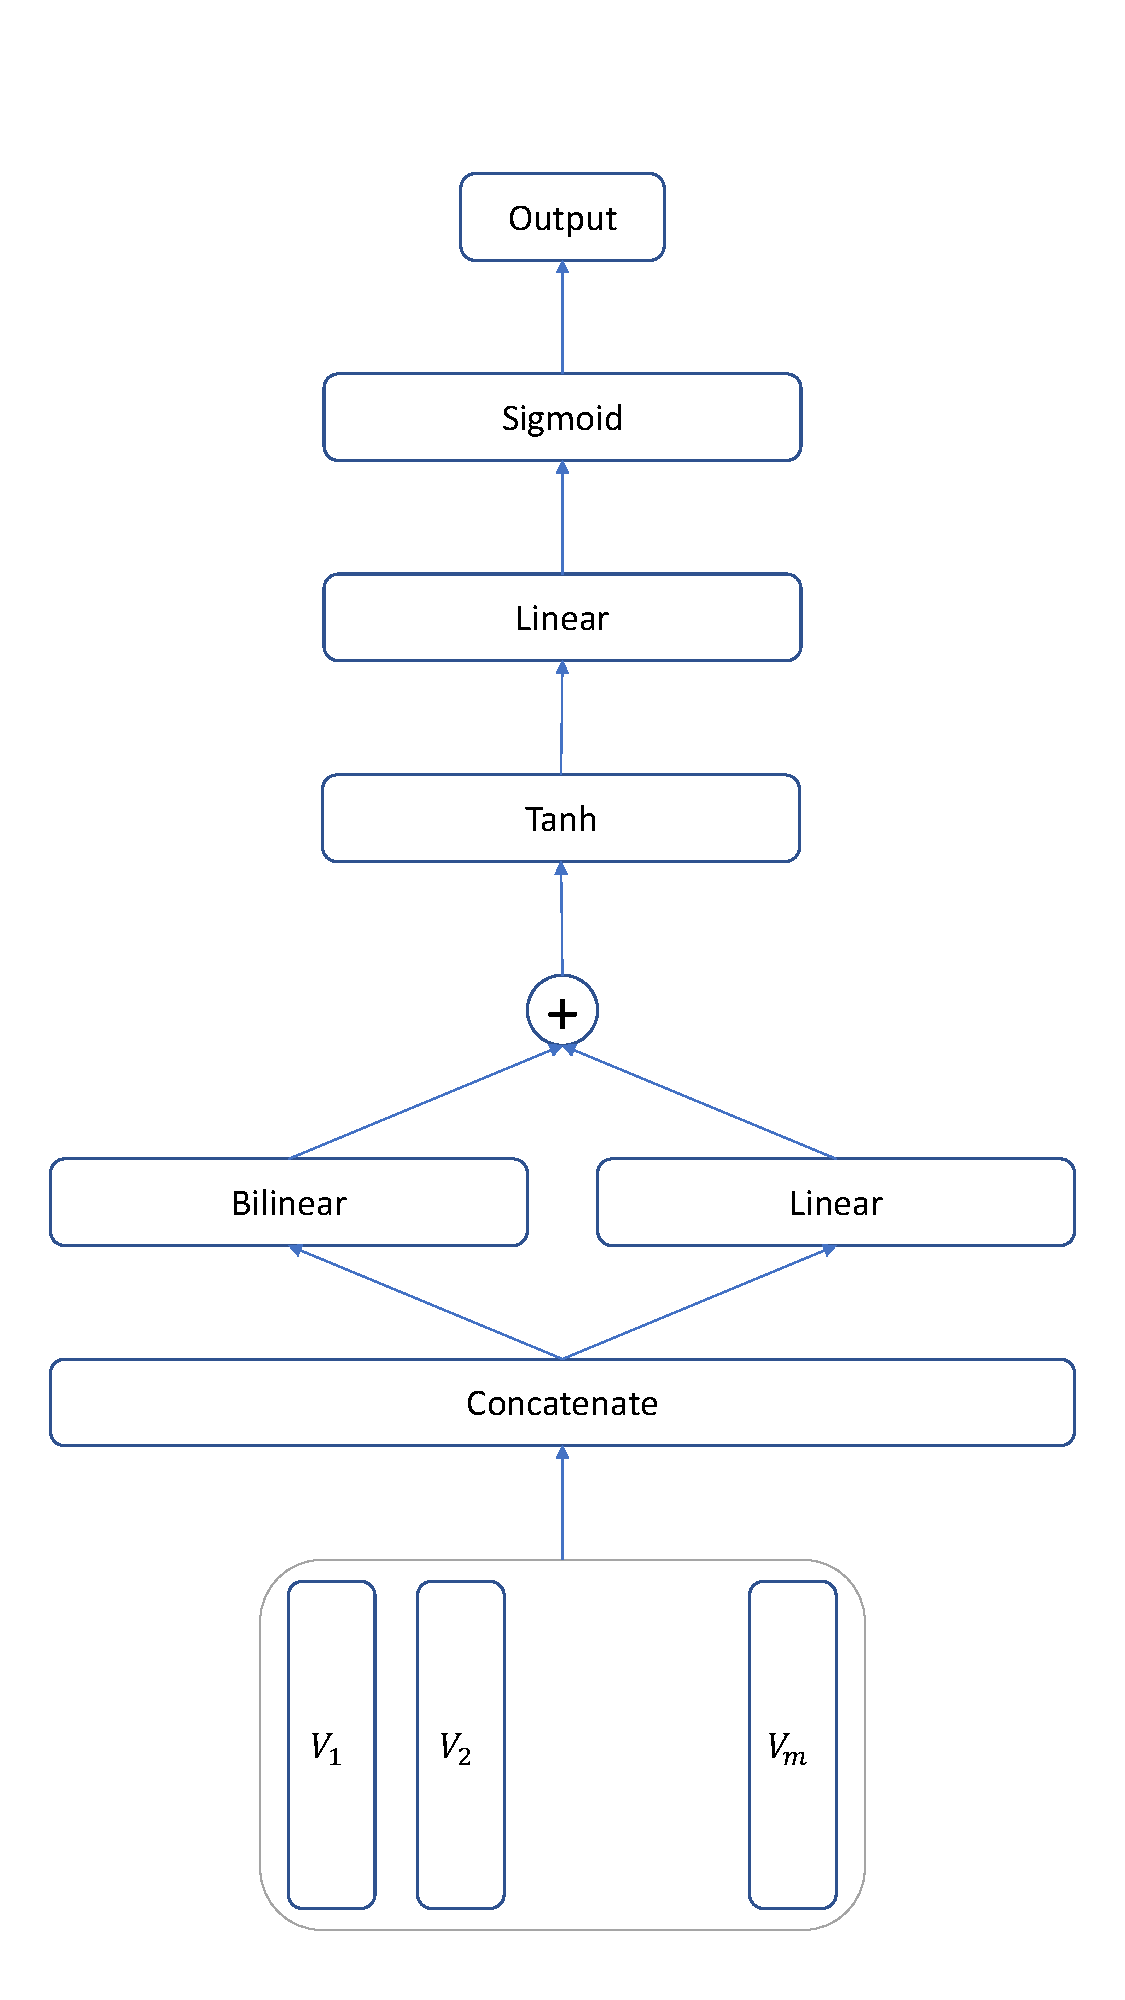
\includegraphics[width=.4\textwidth]{img/Predicate.pdf}
    \caption{Model for Predicate}
    \label{fig:LTN_predicate}
\end{figure}

\subsection{Convolutional Logic Tensor Network (CLTN)}

The model in original LTN is based on classical neural networks. However, recent development on deep learning shows that convolutional neural network (CNN) has more powerful ability. That makes us to extend LTN with CNN.

Here we first follow up the implementation of $G(c)$, $G(f)$, and $G(\phi)$. However, we tend to use Convolutional Neural Network to implement $G(p)$.

First we need to construct the input matrix with the $v_1,v_2,\dots,v_m$. From LTN model, we learned that the bilinear manipulation is critical to get a good performance. Here we construct this bilinear function directly using input vectors of constants. That is, suppose we get $m$ vectors called $x=[v_1,\dots,v_m]$, then $x\in \mathbb{R}^{k\times m}$, where $k$ is the dimension of constant vectors. Therefore, $x^Tx \in \mathbb{R}^{m\times m}$ a squre matrix, which can be treated as a 1-channel image.

The following step is trivial and the model is illustrated in Figure \ref{fig:CLTN_predicate}

\begin{figure}
    \centering
    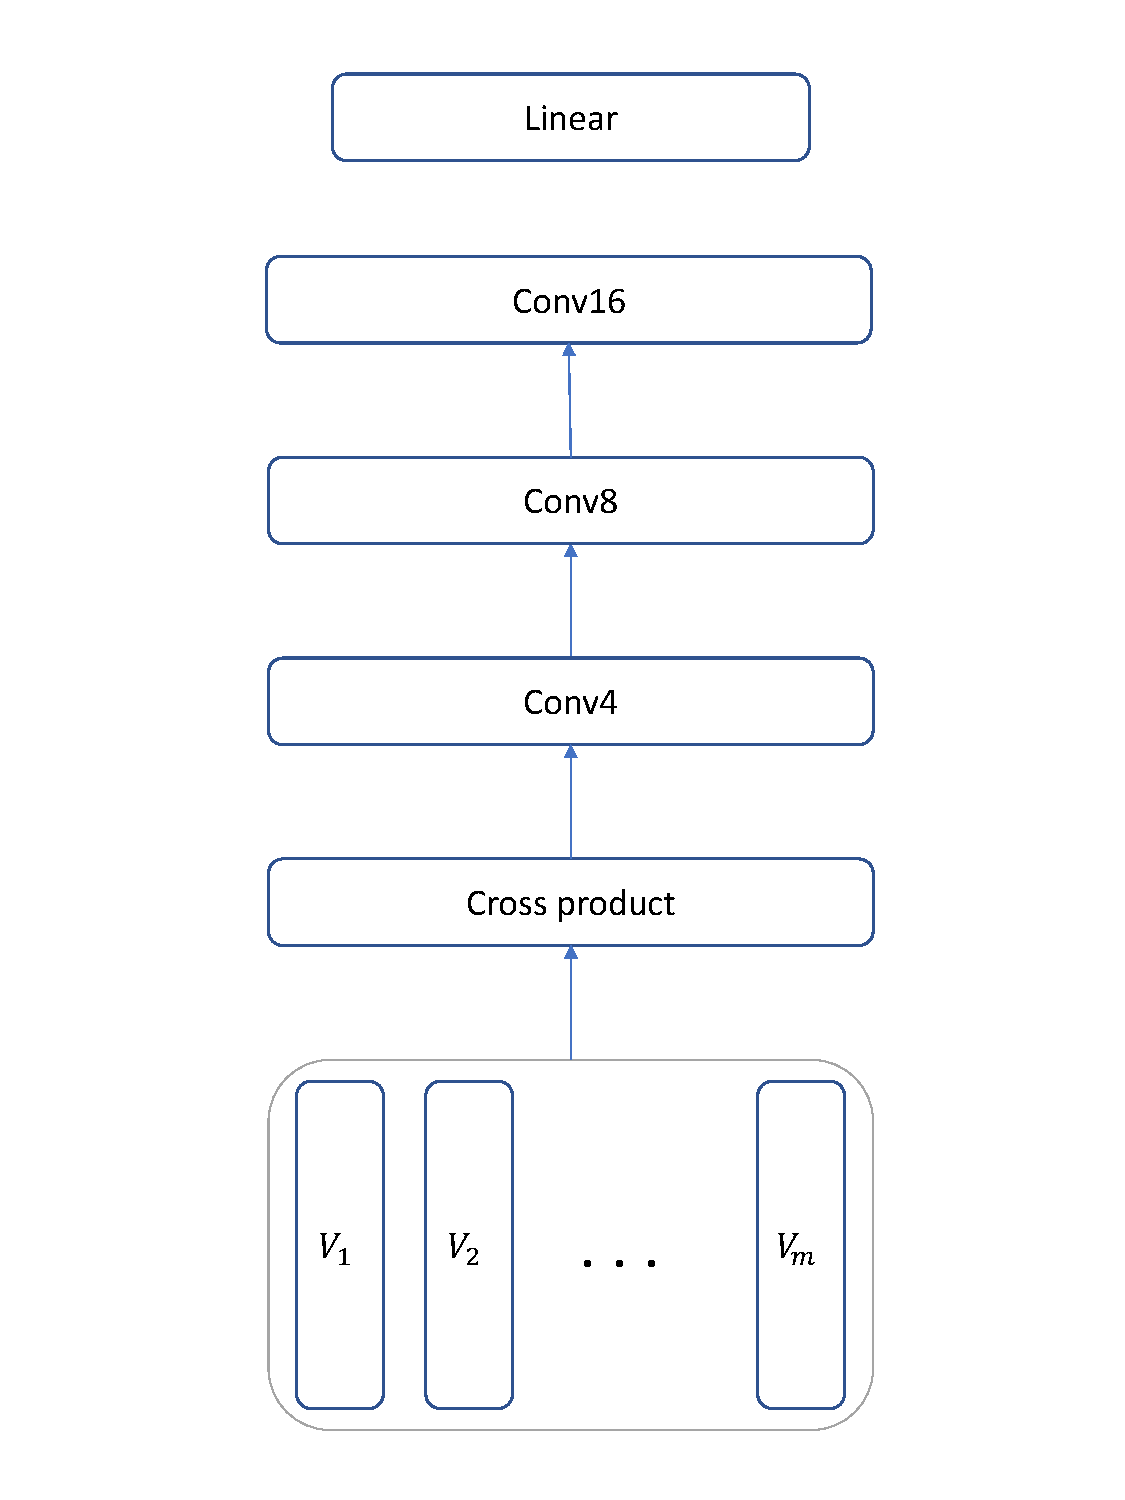
\includegraphics[width=.4\textwidth]{img/CLTN_Predicate.pdf}
    \caption{Model for Predicate}
    \label{fig:CLTN_predicate}
\end{figure}
